\subsection{Using CG to solve the electrostatic problem}

\begin{figure}[!hbt]
    \centering
    \includegraphics[width=0.8\textwidth]{phi_heatmap}
    \caption{The heatmap plot for the solution \(\bm{\phi}\) to
        Equation~\eqref{eq:poissoncorrected} on a \(129 \times 129\) grid,
        after \(500\) CG iterations.}
    \label{fig:phi_heatmap}
\end{figure}

To solve the problem, we need to change the
code in Snippets~\ref{lst:cg} to satisfy the boundary conditions, which includes
the boundary of the whole region and the internal square.

In the beginning, we need to set the initial values of
\(\bm{\phi}(i) = \bm{\phi}(0) = \bm{x}_0\),
where \(i\) labels the number of iterations, as shown in Figure~\ref{fig:t0:a}.
We also need to set the initial values of the residual
%
\begin{equation}\label{eq:r0}
    \bm{r}_0 = \bm{b} - \mathrm{A} \bm{x}_0.
\end{equation}
%
On the boundary and in the internal square, \(\bm{r}_0(x, y)\) is \(0\).
Or, we could just set \(\bm{p}_0(x, y) \equiv 0\) since \(\bm{p}_0 = \bm{r}_0\).

As we start our iterations, we first need to set \(\bm{p}_i(x, y)\) to \(0\)
for \((x, y)\) on the boundary or in the internal square.

The next step is \code{A𝐩ᵢ = A * 𝐩ᵢ}, we also want to set \code{A𝐩ᵢ} to be \(0\)
in these regions. Since \code{A𝐩ᵢ} is used to update the residual:
%
\begin{equation}\label{eq:ri}
    \bm{r}_{i+1} = \bm{r}_i - \alpha_i \mathrm{A} \bm{p}_i.
\end{equation}
%
If \code{A𝐩ᵢ} is not zero in these areas, the residual will grow exponentially
as we iterate.

If these values are set correctly, the residuals \(\{\bm{r}_i\}\) will have
zeros in these regions throughout the whole process.
This is because the values of \(\{\bm{r}_i\}\) (where \(i = 1\), \(\ldots\), \(I\))
only depend on \(\bm{r}_0\) and \(\mathrm{A} \bm{p}_i\), as shown in
Equations~\eqref{eq:r0} and~\eqref{eq:ri}.

\begin{figure}[!hbt]
    \centering
    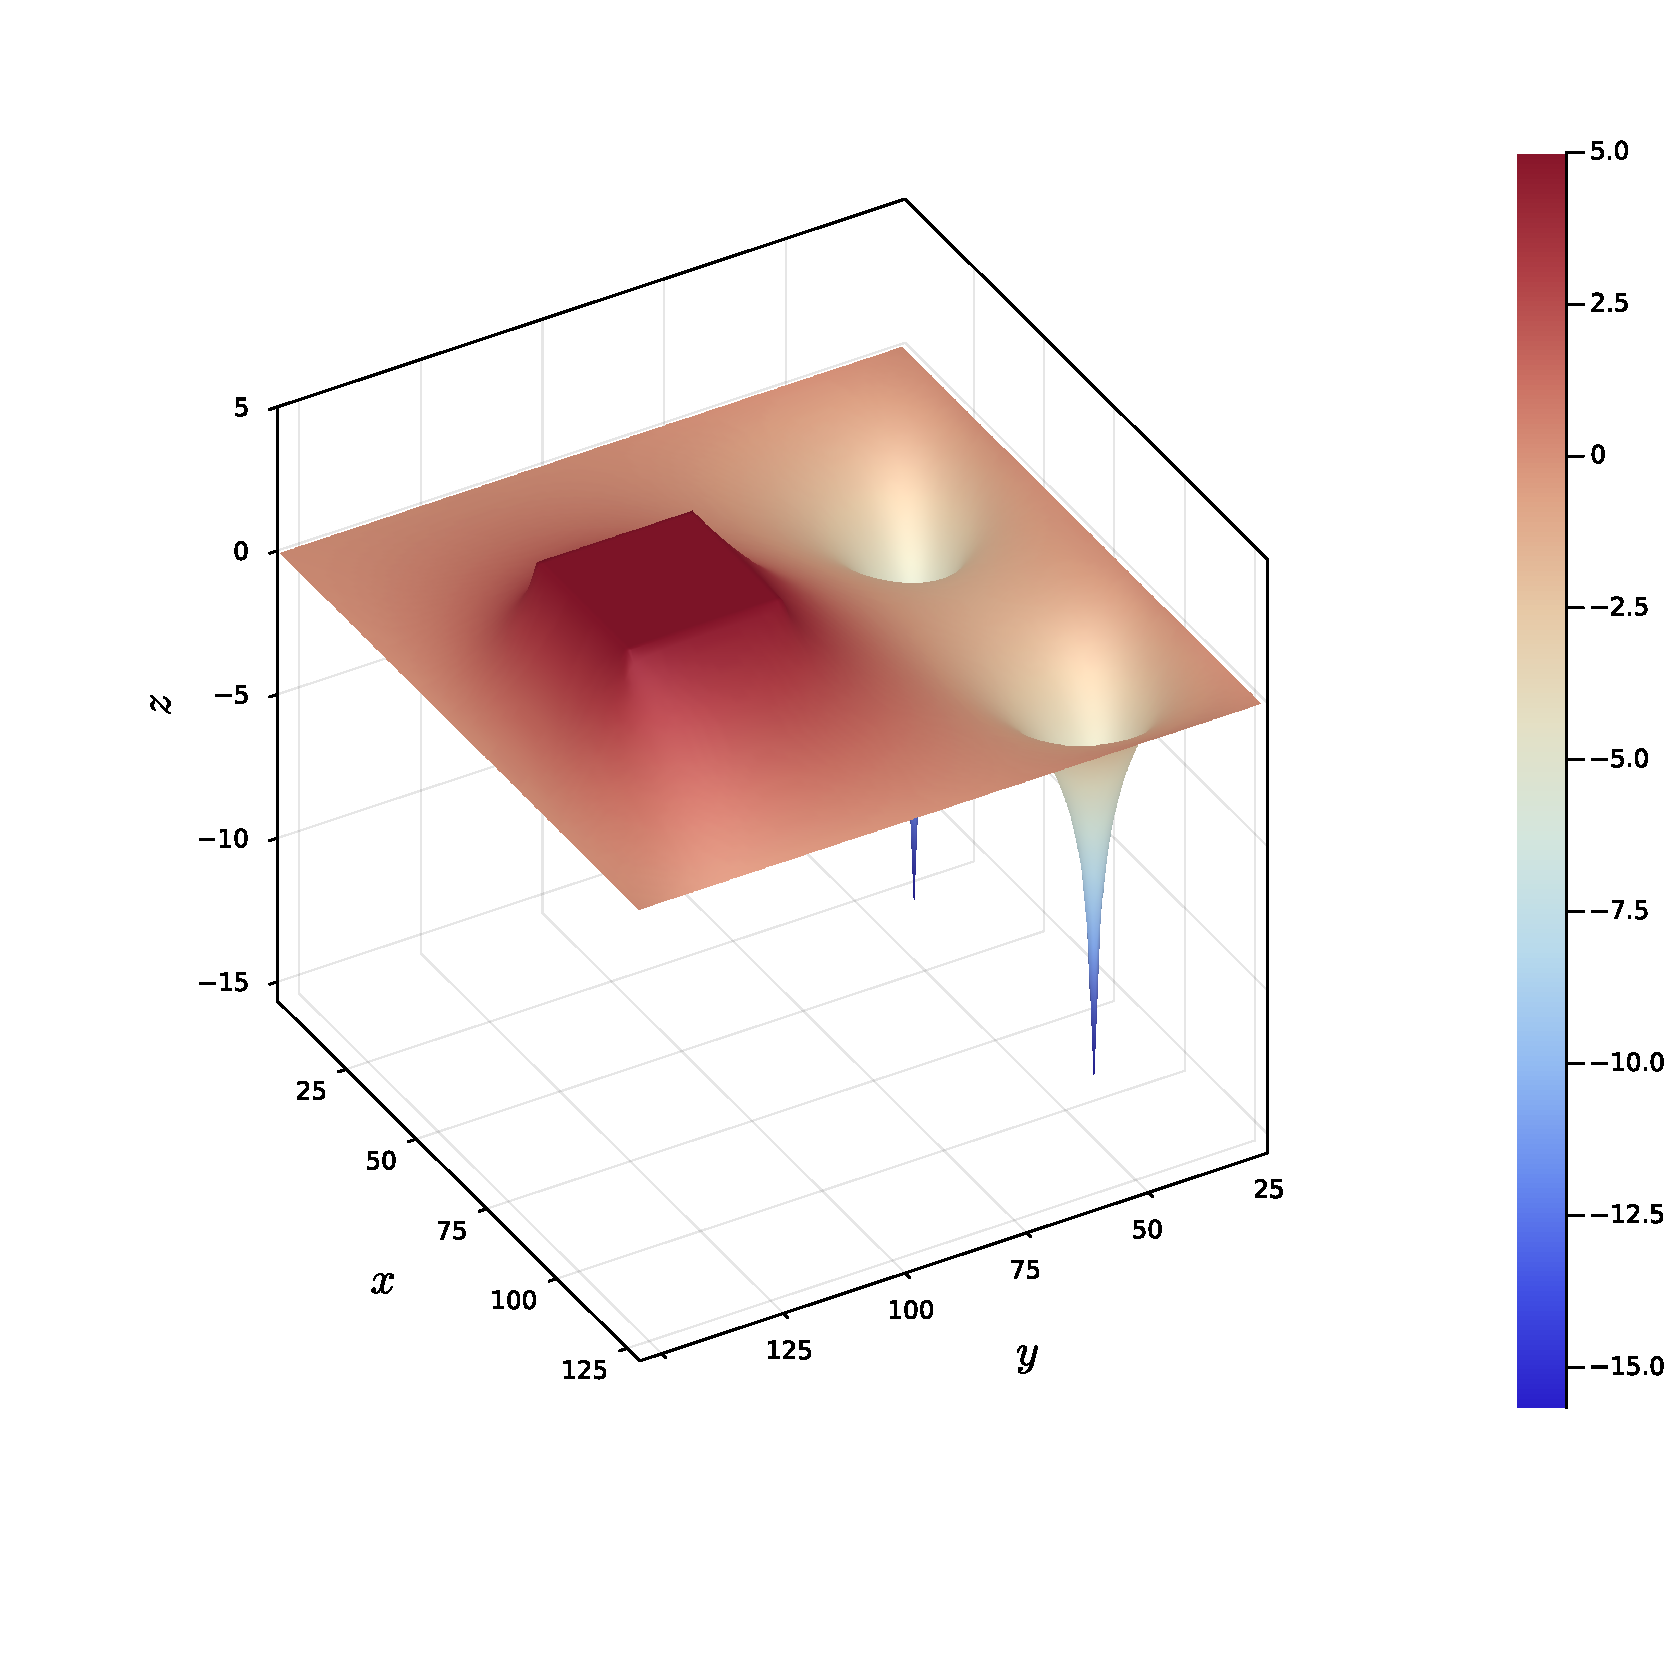
\includegraphics[width=0.8\textwidth]{phi_surface}
    \caption{The surface plot for the solution \(\bm{\phi}\) to
        Equation~\eqref{eq:poissoncorrected} on a \(129 \times 129\) grid,
        after \(500\) CG iterations.}
    \label{fig:phi_surface}
\end{figure}

Also, the values of the solutions, i.e., the electric potential \(\{\bm{\phi}_i\}\),
only depend on its initial value \(\bm{\phi}_0\) and \(\bm{p}_i\) since
%
\begin{equation}
    \bm{x}_{i+1} = \bm{x}_i + \alpha_i \bm{p}_i.
\end{equation}
%
We can check their values as we iterate over \(1\) to \(I\).

\begin{figure}[!hbt]
    \centering
    \includegraphics[width=0.8\textwidth]{residual}
    \caption{The norm of the residual as a function of the number of iterations for solving
        Equation~\eqref{eq:poissoncorrected} on a \(129 \times 129\) grid.
        The \(y\)-axis is in logarithmic scale.}
    \label{fig:residual}
\end{figure}

The solution, \(\bm{x}_I = \bm{\phi}_I\), after \(I=500\) iterations, is reshaped
as a square and plotted as a heatmap in Figure~\ref{fig:phi_heatmap}.
We can see that the negative charges produce negative potentials,
and the highest value for the whole electric potential is at the surface
of the square, as expected.

We also plot a three-dimensional manifold for \(\bm{\phi}_I\)
in Figure~\ref{fig:phi_surface}.
As we can see, at those point charges, the potential decreases drastically,
whose lowest value here is \(-15.661696\).
In fact, if we have a smaller grid size, e.g., \(L = 32\) or \(L = 64\),
we will have a little bit higher values for the minimum of the potential.
Since the \(1 / r\) tail is smeared out by our coarse grid size.

We also plot the norm of the residual as a function of the number of iterations
\(\bm{r}(i)\) in Figure~\ref{fig:residual}. It can be observed how drastically
the residual is decreasing as we iterate.
At the last iteration, the norm of the residual is around \(3.2 \times 10^{-10}\),
which is already negligible in our problem.
